%versi 2 (8-10-2016)
\chapter{Landasan Teori}
\label{chap:teori}

Bab ini membahas tentang landasan teori yang digunakan dalam skripsi ini. Landasan teori yang digunakan, diambil dari dua sumber, yaitu "\textit{CodeIgniter Documentation}" karya \textit{British Columbia Institute of Technology} ~\cite{bcit:17:cidoc} dan "\textit{Sharif Judge Documentation}" karya Mohammad Javad Naderi ~\cite{mjnaderi:14:sharifjudgedoc}.

\section{\textit{CodeIgniter}}
\label{sec:codeigniter} 
 
\textit{CodeIgniter} merupakan sebuah \textit{framework} bagi pengguna yang ingin membangun aplikasi web menggunakan PHP. Tujuan utamanya adalah memungkinkan para pengguna untuk mengembangkan proyek-proyek menjadi lebih cepat dibandingkan menulis kode dari awal. \textit{Framework} ini memiliki banyak libary untuk fungsi-fungsi yang biasa diperlukan, serta antarmuka dan struktur logis yang sederhana untuk mengakses library ini. \textit{CodeIgniter} membuat para pengguna lebih fokus pada proyek dengan cara meminimalkan jumlah kode yang dibutuhkan~\cite{bcit:17:cidoc}. \\

Beberapa keunggulan dari \textit{CodeIgniter} yaitu:
\begin{itemize}
	\item \textit{Framework} yang Ringan \\
		Inti dari sistem \textit{CodeIgniter} membutuhkan \textit{library} yang kecil. Hal ini sangat berbeda dengan \textit{framework} lain yang membutuhkan \textit{resource} lebih. \textit{Library} tambahan dimuat secara dinamis atau sesuai dengan permintaan sehingga sistem dapat berjalan cepat.
	\item Menggunakan Konsep M-V-C \\
		\textit{CodeIgniter} menggunakan pendekatan \textit{Model-View-Controller} yang memungkinkan pemisahan anatara logika dan presentasi.
	\item Menghasilkan \textit{Clean URLs} \\
		\textit{CodeIgniter} menghasilkan \textit{Clean URLs} dan \textit{search-engine friendly}. \textit{Clean URLs} akan mempermudah pengguna dalam membaca \textit{URL}. Contoh perbandingan \textit{URL} biasa dengan \textit{Clean URL}s: \textit{URL} biasa: \path{\\example.com\index.php?page=news}, \textit{Clean URLs}: \path{\\example.com\news}.
	\item \textit{Packs a Punch} \\
		\textit{CodeIgniter} dilengkapi dengan \textit{library} yang umumnya diperlukan untuk mengembangkan \textit{web}, seperti mengakses \textit{database}, mengirim \textit{email}, memvalidasi data \textit{form}, menjaga \textit{session}, memanipulasi gambar dan masih banyak lagi.
	\item \textit{Extensible} \\
		Sistem dapat dengan mudah diperluas dengan menggunakan \textit{library} pengguna, \textit{helper}, atau melalui \textit{class extensions} dan \textit{system hooks}.
	\item Dokumentasi yang Baik \\
		Dokumentasi merupakan salah satu bagian terpenting dari kode itu sendiri. \textit{CodeIgniter} berkomitmen membuat kode yang sangat bersih dan terdokumentasi dengan baik. 
\end{itemize}

\subsection{Fitur-fitur CodeIgniter}
Berikut beberapa fitur utama yang terdapat pada \textit{framework CodeIgniter} seperti:
\begin{itemize}
	\item Sistem berbasis \textit{MVC}
	\item \textit{Framework} yang ringan
	\item \textit{Database Class} yang lengkap dengan dukungan untuk beberapa platform
	\item Dukungan \textit{query builder} untuk database
	\item \textit{Form} dan validasi data
	\item Keamanan dan \textit{XSS Filtering}
	\item \textit{Session Management}
	\item \textit{Email Sending Class}
	\item \textit{Image Manipulation Library}
	\item \textit{File Uploading Class} 
	\item \textit{Calendaring Class}
	\item \textit{Unit Testing Class}
\end{itemize}

\subsection{\textit{Flow Chart} Aplikasi}
Gambar~\ref{fig:flow} menunjukan bagaimana data mengalir ke seluruh sistem~\cite{bcit:17:cidoc}:
\begin{figure}[H]
	\centering  
	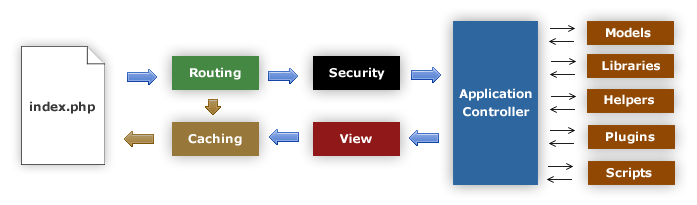
\includegraphics[width=1.0\textwidth]{appflowchart}  
	\caption[\textit{Flow Chart} Aplikasi]{\textit{Flow Chart} Aplikasi} 
	\label{fig:flow} 
\end{figure} 

\begin{enumerate}
	\item File \textit{index.php} berfungsi sebagai \textit{front controller} dan menginisialisasi \textit{resource} utama yang dibutuhkan untuk menjalankan \textit{CodeIgniter}.
	\item \textit{Router} memeriksa \textit{HTTP request} untuk menentukan apa yang harus dilakukan.
	\item Jika terdapat \textit{file cache}, maka akan langsung dikirimkan ke \textit{browser}.
	\item \textit{HTTP request} dan data pengguna yang dikirim akan terlebih dahulu disaring untuk alasan keamanan. \textit{Application controller} akan dimuat setelah proses penyaringan selesai.
	\item \textit{Controller} akan memuat \textit{model, core libraries, helpers} dan \textit{resource} lain yang dibutuhkan untuk memproses permintaan khusus.
	\item \textit{View} akan di \textit{render} kemudian dikirim ke web \textit{browser}. Jika proses \textit{caching} diaktifkan, maka \textit{View} akan di \textit{cache} terlebih dahulu sehingga permintaan berikutnya dapat dilayani.
\end{enumerate}

\subsection{\textit{Model-View-Controller}}
\textit{CodeIgniter} merupakan \textit{framework} yang menggunaakan pola pengembangan \textit{Model-View-Controller}. \textit{MVC} adalah pendekatan perangkat lunak yang memisahkan logika aplikasi dari presentasi. Hal tersebut memungkinkan halaman web pengguna memiliki \textit{scripting} yang sedikit karena presentasi terpisah dari \textit{scripting} PHP~\cite{bcit:17:cidoc}. \\

	\subsubsection{\textit{Model}}
	\textit{Model} merepresentasikan bagian struktur data pengguna. Biasanya kelas \textit{Model} berisikan fungsi-fungsi yang membantu pengguna untuk mengambil, menyimpan, dan memperbarui informasi pada \textit{database}. Berikut beberapa hal penting yang terdapat pada \textit{Model}:
	\begin{itemize}
		\item Susunan dari \textit{Model} \\
		Kelas \textit{model} berada di direktori \path{application/models/}. \textit{Model} dapat dikelompokkan di dalam sub direktori jika pengguna menginginkannya. Bentuk dasar kode pada kelas \textit{model} digambarkan seperti berikut ini:
		\begin{lstlisting}[basicstyle=\ttfamily, frame=single,
columns=fullflexible, keepspaces=true, breaklines=true]
class Model_name extends CI_Model {
	public function_construct()
	{
		parent::_construct();
		//constructor code
	}
}
\end{lstlisting}
		
		\textit{Model\_name} adalah nama kelas dari kelas \textit{model} yang pengguna buat. Penamaan kelas harus dimulai dengan huruf kapital. Pastikan kelas \textit{model} merupakan turunan dari \textit{base Model} (\textit{class CI\_Model} atau \textit{MY\_Model}).
		
		\item Menghubungkan Sebuah \textit{Model} \\
		Pada dasarnya \textit{model} akan dimuat dan dipanggil dari \textit{method} atau fungsi yang ada pada \textit{controller}. Untuk menghubungkan \textit{model}, pengguna harus menggunakan method berikut:
		\begin{lstlisting}[basicstyle=\ttfamily, frame=single,
columns=fullflexible, keepspaces=true, breaklines=true]
$this->load->model('model_name');
\end{lstlisting}
		
		Jika \textit{model} yang pengguna buat terletak di dalam sebuah sub-direktori, maka pengguna harus menyertakan alamat relatif \textit{(relative path)} dari \textit{model} yang dibuat. Sebagai contoh, jika \textit{model} yang pengguna berlokasi di \path{application/models/blog/Queries.php} pengguna dapat menghubungkannya dengan cara:
		\begin{lstlisting}[basicstyle=\ttfamily, frame=single,
columns=fullflexible, keepspaces=true, breaklines=true]
$this->load->model('blog/queries');
\end{lstlisting}
		
		Pengguna dapat mengakses \textit{method} yang terdapat pada \textit{model} menggunakan sebuah objek dengan nama yang sama dengan nama kelas yang pengguna buat sebelumnya:
		\begin{lstlisting}[basicstyle=\ttfamily, frame=single,
columns=fullflexible, keepspaces=true, breaklines=true]
$this->load->model('model_name');
		
$this->model_name->method();
\end{lstlisting}
		
		Jika pengguna ingin menggunakan objek yang berbeda untuk sebuah \textit{model}, maka pengguna dapat menggunakan penamaan (alias) di parameter kedua:
		\begin{lstlisting}[basicstyle=\ttfamily, frame=single,
columns=fullflexible, keepspaces=true, breaklines=true]
$this->load->model('model_name', 'foobar');
	
$this->foobar->method();
\end{lstlisting}
		
		Berikut merupakan contoh sebuah \textit{controller} yang terhubung dengan sebuah \textit{model} dan menampilkan data hasil olahan \textit{model} ke \textit{view}:
		\begin{lstlisting}[basicstyle=\ttfamily, frame=single,
columns=fullflexible, keepspaces=true, breaklines=true]
class Blog_controller extends CI_Controller {
			
	public function blog()
	{
		$this->load->model('blog');
		
		$data['query'] = $this->blog->data_sepuluh
		_artikel_terakhir();
		
		$this->load->view('blog', $data);
	}
}
\end{lstlisting}
		
		\item \textit{Auto-loading Model} \\
		\textit{Auto-loading} (menghubungkan secara otomatis) model tertentu secara global dapat pengguna lakukan dengan menggunakan pengaturan yang ada pada berkas \path{application/config/autoload.php}. Kode yang ditambahkan untuk menghubungkan \textit{model} secara otomatis selama sistem berjalan adalah \textit{\$autoload['model'] = array('model\_name');}
		
		\item Koneksi ke \textit{Database} \\
		Ketika sebuah \textit{model} dipanggil, \textit{model} tidak akan terhubung ke \textit{database} secara otomatis. Beberapa opsi yang dapat digunakan untuk menghubungkan \textit{model} ke \textit{database}:
		\begin{itemize}
			\item Pengguna dapat menghubungkan dengan menggunakan metode standar \textit{database} antara \textit{class Controller} atau \textit{class Model}. \\
			\item Pengguna dapat mengatur sebuah \textit{model} melakukan \textit{auto-connect} dengan menambahkan nilai \textit{TRUE} (boolean) di parameter ketiga atau mengatur konektivitas sebagaimana yang telah didefinisikan di dalam \textit{file} \path{application/config/database.php}
			\begin{lstlisting}[basicstyle=\ttfamily, frame=single,
columns=fullflexible, keepspaces=true, breaklines=true]
$this->load->model('model_name', '', TRUE);
\end{lstlisting}
			\item Pengguna dapat mengatur koneksi secara manual dengan menambahkan \textit{item-item} berupa \textit{array} pada \textit{parameter} ketiga seperti contoh berikut:
			\begin{lstlisting}[basicstyle=\ttfamily, frame=single,
columns=fullflexible, keepspaces=true, breaklines=true]
$config['hostname'] = 'localhost';
$config['username'] = 'username';
$config['password'] = 'katasandi';
$config['database'] = 'database_name';
$config['dbdriver'] = 'mysqli';
$config['dbprefix'] = '';
$config['pconnect'] = FALSE;
$config['db_debug'] = TRUE;
			
$this->load->model('model_name', '', $config);
\end{lstlisting}
		\end{itemize}
	\end{itemize}
	
	\subsubsection{\textit{View}}
	\textit{View} merupakan informasi yang akan ditampilkan kepada pengguna. Umumnya \textit{View} merupakan sebuah halaman web, namun pada \textit{CodeIgniter}, \textit{View} dapat berupa bagian-bagian halaman seperti \textit{header} atau \textit{footer}. Selain itu \textit{View} juga dapat berupa halaman \textit{RSS} atau jenis "halaman" lainnya. \textit{View} tidak pernah dipanggil secara langsung, melainkan harus melalui \textit{controller} karena dalam \textit{framework} \textit{MVC}, \textit{controller} berfungsi sebagai pengatur. Untuk memuat tampilan tertentu, pengguna dapat menggunakan \textit{method} berikut:
	\begin{lstlisting}[basicstyle=\ttfamily, frame=single,
columns=fullflexible, keepspaces=true, breaklines=true]
$this->load->view('name');
\end{lstlisting}
	
	\textit{CodeIgniter} dapat menangani beberapa panggilan \textit{method} \textit{\$this->load->view()} dari dalam \textit{controller}. Jika lebih dari satu panggilan terjadi, maka panggilan tersebut ditambahkan bersama. Contohnya pengguna ingin memiliki \textit{header view, menu view, content view} dan \textit{footer view}. Kode program yang digunakan seperti berikut:
	\begin{lstlisting}[basicstyle=\ttfamily, frame=single,
columns=fullflexible, keepspaces=true, breaklines=true]
class Page{
	public function INDEX(){
		$data['page_title'] = 'Your title';
		$load->view('header');
		$load->view('menu');
		$load->view('content', $data);
		$load->view('footer');
	}
}
\end{lstlisting}
	
	\subsubsection{\textit{Controller}}
	\textit{Controller} berfungsi sebagai perantara antara \textit{Model}, \textit{View} dan \textit{resource} lain yang dibutuhkan untuk memproses \textit{HTTP request} dan menghasilkan halaman web. Controller merupakan sebuah kelas yang dinamakan demikian agar dapat dikaitkan dengan URI. Sebagai contoh URI \path{example.com/index.php/blog/}, \textit{CodeIgniter} akan mencari \textit{controller} bernama \textit{Blog.php} dan menjalankannya. Nama \textit{cont}roller harus diawali dengan huruf kapital. Selain itu controller juga harus \textit{extend} kelas "\textit{CI\_Controller}".
	Perhatikan contoh berikut:\\
	Contoh yang benar :
\begin{lstlisting}[basicstyle=\ttfamily, frame=single,
columns=fullflexible, keepspaces=true, breaklines=true]
<?php
class Blog extends CI_Controller {

}
\end{lstlisting}
	
	Contoh yang salah :
\begin{lstlisting}[basicstyle=\ttfamily, frame=single,
columns=fullflexible, keepspaces=true, breaklines=true]
<?php
class blog extends CI_Controller {

}
\end{lstlisting} 

	Berikut beberapa hal penting yang terdapat pada \textit{Controller}:
	\begin{itemize}
		\item \textit{Method} \\
		Untuk menjalankan suatu \textit{method}, pengguna perlu menuliskannya pada segmen kedua URI. Perhatikan contoh berikut:
\begin{lstlisting}[basicstyle=\ttfamily, frame=single,
columns=fullflexible, keepspaces=true, breaklines=true]
<?php
class Blog extends CI_Controller {
		public function index()
		{
			echo 'Hello World!';
		}
		
		public function comments()
		{
			echo 'Look at this!';
		}
		
		public function shoes($sandals, $id)
		{
			echo $sandals;
			echo $id;
		}
}
\end{lstlisting}
		Jika pengguna memuat URL \path{example.com/index.php/blog/comments}, maka method \textit{comments()} akan dijalankan pada \textit{controller} \textit{Blog.php}. \textit{Method index()} akan dijalankan jika bagian kedua URI kosong. Jika URI mengandung lebih dari dua segment, maka segmen-segmen tersebut akan dimasukan ke dalam \textit{method} sebagai parameter. Contoh: pengguna memuat URL \path{example.com/index.php/blog/shoes/sandals/123}. Segmen "\textit{sandals}" dan "123" akan dimasukan sebagai \textit{parameter} ke dalam \textit{method shoes}.
		
		\item \textit{Default Controller} \\
		\textit{CodeIgniter} dapat diperintahkan untuk menjalankan \textit{default controller} jika tidak terdapat URI. Hal ini umumnya terjadi ketika terdapat permintaan menggunakan URL dasar \textit{website}. Penentuan \textit{default controller} terdapat pada \textit{file} \path{application/config/routes.php}. Perhatikan contoh berikut:
\begin{lstlisting}[basicstyle=\ttfamily, frame=single,
columns=fullflexible, keepspaces=true, breaklines=true]
$route['default_controller'] = 'blog';
\end{lstlisting} 
		\textit{Blog} merupakan nama kelas \textit{controller} yang ingin digunakan. Jika pengguna mengakses file \textit{index.php} utama tanpa menentukan segmen URI, maka akan dijalankan \textit{controller} \textit{Blog}.
		
%		\item \textit{Processing Output} \\
%		\textit{CodeIgniter} memiliki kelas \textit{output} yang menangani pengiriman data ke \textit{web browser} secara otomatis. Dalam beberapa kasus saat pengguna ingin mengubah cara pengiriman data tersebut, CodeIgnite\textit{}r akan menambahkan \textit{method} bernama "\_output()" ke \textit{controller} terkait. Jika controller memiliki method bernama "\_output()" maka controller tersebut akan selalu dipanggil oleh kelas "\textit{output}".
%		Contoh penggunaan method "\_output()" : 
%\begin{lstlisting}[basicstyle=\ttfamily, frame=single,
%columns=fullflexible, keepspaces=true, breaklines=true]
%public function _output(\$output)
%{
%	echo $output;
%}
%\end{lstlisting}
		
		\item \textit{Private Method}\\
		\textit{Method-method} dengan tipe \textit{private} tidak dapat diakses oleh publik. \textit{Method} ini hanya dapat diakses oleh \textit{method} lain dalam \textit{controller} yang sama dan \textit{method} ini juga tidak dapat diakses melalui URL. Contoh penulisan \textit{private method}:
		\begin{lstlisting}[basicstyle=\ttfamily, frame=single,
columns=fullflexible, keepspaces=true, breaklines=true]
private function _utility()
{
	// kode program
}
\end{lstlisting}
		
		\textit{Method} di atas tidak dapat diakses dengan cara pemanggilan method yang umum seperti berikut:
		\begin{lstlisting}[basicstyle=\ttfamily, frame=single,
columns=fullflexible, keepspaces=true, breaklines=true]
example.com/index.php/blog/_utility/
\end{lstlisting}
		
		\item Mengorganisir \textit{Controller} ke Dalam Sub Direktori \\
		\textit{CodeIgniter} mengizinkan pengguna untuk mengorganisir \textit{controller} ke dalam sub direktori. Pengguna dapat membuat sub direktori di dalam direktori \path{application/controllers/} dan menyimpan kelas \textit{controller} ke direktori tersebut. Ketika menggunakan fitur ini, pengguna harus menspesifikasikan folder tersebut ke dalam URI. Perhatikan contoh berikut:
		Sebuah \textit{controller} berlokasi pada direktori \path{application/controllers/products/Shoes.php}. Untuk memanggil controller tersebut, URI pengguna yang tampil akan seperti \path{example.com/index.php/products/shoes/show/123}.
	\end{itemize}

%\textit{CodeIgniter} memiliki pendekatan yang cukup fleksibel terhadap \textit{MVC} karena \textit{Model} tidak selalu diperlukan. Para pengguna dapat membangun aplikasi hanya menggunakan \textit{Controller} dan \textit{View}. Hal tersebut dapat dilakukan jika pengguna tidak memerlukan adanya pemisahan tambahan atau pengguna merasa bahwa menggunakan sebuah \textit{Model} membutuhkan kompleksitas yang lebih tinggi~\cite{bcit:17:cidoc}. 

\subsection{Desain dan Tujuan Arsitektur}
Dari sudut pandang teknis dan arsitektural, \textit{CodeIgniter} dibuat dengan tujuan sebagai berikut:
\begin{itemize}
	\item \textit{Dynamic Instation} \\
	Dalam \textit{CodeIgniter}, komponen dimuat dan dieksekusi jika diminta. Tidak ada asumsi yang dibuat oleh sistem tentang apa yang mungkin diperlukan di luar \textit{resource} utama, sehingga sistem sangat ringan secara \textit{default}. \textit{Event}, \textit{Controller} dan \textit{View} yang pengguna rancang akan menentukan apa yang dipanggil.
	\item \textit{Loose Coupling} \\
	\textit{Coupling} adalah sejauh mana komponen-komponen dari sistem saling mengandalkan satu sama lain. Semakin sedikit komponen yang bergantung satu sama lain, maka komponen tersebut lebih dapat digunakan kembali dan sistem menjadi lebih fleksibel. Tujuan dari \textit{framework} ini adalah sistem yang sangat longgar (\textit{very loosely coupled system}).
	\item \textit{Component Singularity} \\
	\textit{Singularity} adalah sejauh mana komponen memiliki tujuan. Dalam CodeIgniter, setiap kelas dan fungsinya sangat otonom. Hal tersebut memungkinkan fungsi dapat berjalan secara maksimal.
\end{itemize}

\textit{CodeIgniter} merupakan sistem yang \textit{loosely coupled} dengan singularitas komponen yang tinggi (\textit{dynamically instantiated}). \textit{Codeigniter} berusaha untuk sederhana, fleksible dan kinerja tinggi dengan paket yang sekecil mungkin ~\cite{bcit:17:cidoc}.

\section{\textit{Sharif Judge}}
\label{sec:sharifjudge} 

\textit{Sharif Judge} adalah \textit{grader} otomatis yang mampu menilai ketepatan serta performansi program yang dikumpulkan mahasiswa. Perangkat lunak ini diciptakan oleh Mohammad Javad Naderi dan bersifat \textit{open source}. Antarmuka \textit{Sharif Judge} ditulis menggunakan bahasa pemrograman PHP (\textit{framework CodeIgniter}) dan \textit{backend} menggunakan \textit{BASH} \cite{mjnaderi:14:sharifjudge}.
Selain sebagai \textit{grader} otomatis, \textit{Sharif Judge} juga memiliki beberapa fitur lainnya seperti:
\begin{itemize}
	\item Beberapa peran (\textit{role}) \textit{users} (\textit{admin, head instructor, instructor, student})
	\item \textit{Sandboxing} (belum diterpakan untuk \textit{phyton})
	\item Deteksi kecurangan (mendeteksi kode yang mirip) menggunakan \textit{Moss}
	\item Pengaturan untuk menilai keterlambatan pengiriman
	\item Antrian Pengiriman
	\item Mengunduh hasil dalam bentuk \textit{file excel}
	\item Mengunduh kode yang telah dikirim dalam bentuk \textit{file zip}
	\item Metode "\textit{Output Comparison}" dan "\textit{Tester Code}" untuk memeriksa kebenaran dari hasil keluaran.
	\item Menambahakan beberapa pengguna sekaligus
	\item Diskripsi \textit{Problem} (\textit{PDF/Markdown/HTML})
	\item Penilaian ulang (\textit{rejudge})
	\item Papan nilai
	\item Notifikasi
\end{itemize}

\subsection{Instalasi}
Untuk menjalankan \textit{Sharif Judge}, dibutuhkan sebuah server \textit{Linux} dengan persyaratan berikut ~\cite{mjnaderi:14:sharifjudgedoc}:
\begin{itemize}
	\item \textit{Webserver} menjalankan PHP versi 5.3 atau yang lebih baru
	\item Pengguna harus dapat menjalankan PHP dari \textit{command line}. Pada \textit{Ubuntu}, pengguna perlu meginstal paket \textit{php5-cli}
	\item \textit{Mysql database} (dengan ekstensi \textit{mysqli} untuk PHP) atau \textit{PostgreSql database}
	\item PHP harus memiliki akses untuk menjalankan \textit{shell commands} menggunakan fungsi \textit{shell\textunderscore exec}. Contohnya seperti \textit{command} di bawah ini: 
		\begin{lstlisting}[basicstyle=\ttfamily, frame=single,
columns=fullflexible, keepspaces=true, breaklines=true]
echo shell_exec("php -v");
\end{lstlisting}
	\item Perkakas yang digunakan untuk \textit{compiling} dan menjalankan kode yang dikumpulkan adalah (\textit{gcc, g++, javac, java, python2, python3 commands})
	\item \textit{Perl} lebih baik diinstal untuk alasan ketepatan waktu, batas memori dan memaksimalkan batas ukuran pada \textit{output} kode yang dikirimkan
\end{itemize}


Jika persyaratan di atas telah terpenuhi, maka akan masuk tahap instalasi sebagai berikut:
\begin{itemize}
	\item Mengunduh versi terakhir dari \textit{Sharif Judge} dan \textit{unpack} hasil download di direktori \textit{public html}
	\item (Pilihan) Pindahkan folder \textit{system} dan \textit{application} keluar dari \textit{public directory} dan
	masukan \textit{path} lengkap di \textit{file index.php} 
	\begin{lstlisting}[basicstyle=\ttfamily, frame=single,
columns=fullflexible, keepspaces=true, breaklines=true]
$system_path = '/home/mohammad/secret/system';
$application_folder = '/home/mohammad/secret/application';
\end{lstlisting}
	\item Buat sebuah \textit{Mysql} atau \textit{PostgreSql} \textit{database} untuk \textit{Sharif Judge}. Jangan menginstall paket koneksi \textit{database} untuk \textit{C/C++, Java}, atau \textit{Python}
	\item Atur pengaturan koneksi \textit{database} di file \path{application/config/database.php}. Pengguna dapat menggunakan awalan untuk nama tabel.
	\begin{lstlisting}[basicstyle=\ttfamily, frame=single,
columns=fullflexible, keepspaces=true, breaklines=true]
/*  Enter database connection settings here:  */
'dbdriver' => 'postgre',    // database driver (mysqli, postgre)
'hostname' => 'localhost',  // database host
'username' => `,           // database username
'password' => `,           // database password
'database' => `,           // database name
'dbprefix' => 'shj_',       // table prefix
/**********************************************/
\end{lstlisting}
	\item Buat direktori \textit{application/cache/Twig} agar dapat ditulis oleh PHP
	\item Buka halaman utama \textit{Sharif Judge} pada web \textit{browser} dan ikuti proses instalasi berikutnya
	\item \textit{Log in} menggunakan akun \textit{admin}
	\item Pindahkan folder \textit{tester} dan \textit{assigments} di luar \textit{public directory} lalu simpan \textit{path} lengkap di halaman \textit{Settings}. Dua folder tersebut harus dapat ditulis oleh PHP. \textit{File-file} yang diunggah akan disimpan di folder \textit{assigments} sehingga tidak dapat diakses publik.
\end{itemize}

\subsection{\textit{Clean URLs}}
Secara \textit{default}, \textit{index.php} merupakan bagian dari seluruh \textit{URLs} yang ada pada \textit{Sharif Judge} seperti~\cite{mjnaderi:14:sharifjudgedoc}:  \\
\path{http://example.mjnaderi.ir/index.php/dashboard} \\
\path{http://example.mjnaderi.ir/index.php/users/add} \\
Pengguna dapat menghilangkan \textit{index.php} dan memiliki \textit{urls} yang baik jika sistem pengguna mendukung aturan \textit{rewrite} seperti: \\ 
\path{http://example.mjnaderi.ir/dashboard}\\
\path{http://example.mjnaderi.ir/users/add}\\
Untuk memungkinkan \textit{clean urls}, ubah isi file \textit{.htaccess2} menjadi \textit{.htaccess} yang berlokasi di direktori utama \textit{Sharif Judge}.
Berikut isi file \textit{.htaccess2}: 
\begin{lstlisting}[basicstyle=\ttfamily, frame=single,
columns=fullflexible, keepspaces=true, breaklines=true]
# You also need to change 
# $config['index_page'] = 'index.php';
# to
# $config['index_page'] = '';
# in application/config/config.php
# in order to enable clean urls.

RewriteEngine on
RewriteCond $1 !^(index\.php|assets|robots\.txt)
RewriteRule ^(.*)$ index.php?/$1 [L]
\end{lstlisting}
Lalu buka file \path{application/config/config.php} dan ubah \textit{\$config['index\_page'] = 'index.php';} menjadi \textit{\$config['index\_page'] = '';}.

\subsection{\textit{Users}}
Pada \textit{Sharif Judge}, \textit{users} dibagi menjadi 4 \textit{role}. Keempat \textit{role} tersebut adalah \textit{Admins, Head Instructor, Instructor, }dan \textit{Students}
Tabel~\ref{tab:userrole} menunjukan \textit{level users}~\cite{mjnaderi:14:sharifjudgedoc}.

\begin{table}[H] %atau h saja untuk "kira kira di sini"
	\centering 
	\caption{\textit{User Roles Table}}
	\label{tab:userrole}
	\begin{tabular}{|c|c|}
		\hline
		\textit{\textbf{User Role}} & \textit{\textbf{User Level}} \\
		\hline
		\textit{Admin} & 3 \\
		\hline
		\textit{Head Instructor} & 2 \\
		\hline
		\textit{Instructor} & 1 \\
		\hline
		\textit{Student} & 0 \\
		\hline		
	\end{tabular} 
\end{table}

Setiap \textit{users} dapat melakukan aksi yang berbeda-beda. Aksi yang dapat dilakukan para \textit{users} akan disesuaikan dengan \textit{level} masing-masing. Perhatikan tabel~\ref{tab:useraction} berikut:
\begin{table}[H] %atau h saja untuk "kira kira di sini"
	\centering 
	\caption{\textit{Permission Table}}
	\label{tab:useraction}
	\begin{tabular}{|l|c|c|c|c|}
		\hline
		Aksi & \textit{Admin} & \textit{Head Instructor} & \textit{Instructor} & \textit{Student} \\
		
		\hline
		Mengubah \textit{Settings} & \ding{51} & \ding{53} & \ding{53} & \ding{53} \\
		Menambah/Menghapus \textit{users} & \ding{51} & \ding{53} & \ding{53} & \ding{53} \\
		Mengubah Peran \textit{users} & \ding{51} & \ding{53} & \ding{53} & \ding{53} \\
		Menambah/Menghapus/Mengubah \textit{Assignment} & \ding{51} & \ding{51} & \ding{53} & \ding{53} \\
		Mengunduh \textit{Test} & \ding{51} & \ding{51} & \ding{53} & \ding{53} \\
		
		Menambah/Menghapus/Mengubah Notifikasi & \ding{51} & \ding{51} & \ding{53} & \ding{53} \\
		\textit{Rejudge} & \ding{51} & \ding{51} & \ding{53} & \ding{53} \\
		Melihat/\textit{Pause}/Melanjutkan/\textit{Submission Queue} & \ding{51} & \ding{51} & \ding{53} & \ding{53} \\
		Mendeteksi Kode yang Mirip & \ding{51} & \ding{51} & \ding{53} & \ding{53} \\
		Melihat Semua Kode & \ding{51} & \ding{51} & \ding{51} & \ding{53} \\
		
		Mengunduh Kode Final& \ding{51} & \ding{51} & \ding{51} & \ding{53} \\
		Memilih \textit{Assignment} & \ding{51} & \ding{51} & \ding{51} & \ding{51} \\
		\textit{Submit} & \ding{51} & \ding{51} & \ding{51} & \ding{51} \\
		
		\hline
		
	\end{tabular} 
\end{table}

Pengguna dapat menambahkan \textit{users} dengan mengklik pada bagian \textit{Add Users} di halaman \textit{Users}. Pengguna harus mengisi semua informasi yang ada pada \textit{text area}. Baris dimulai dengan komentar \textit{\#}. Setiap baris lainnya mewakili pengguna dengan sintaks berikut:
\begin{lstlisting}[basicstyle=\ttfamily, frame=single,
columns=fullflexible, keepspaces=true, breaklines=true]
USERNAME EMAIL PASSWORD ROLE
	
* Usernames dapat berisikan huruf kecil atau nomor dan harus terdiri 
  antara 3 sampai 20 karakter.
* Passwords harus terdiri antara 6 sampai 30 karakter.
* Pengguna dapat menggunakan RANDOM[n] untuk menghasilkan password 
  acak yang terdiri dari n-digit karakter.
* ROLE harus terdiri dari salah satu ini: `admin`, `head_instructor`, 
  `instructor`, `student`
\end{lstlisting}
Contoh:
\begin{lstlisting}[basicstyle=\ttfamily, frame=single,
columns=fullflexible, keepspaces=true, breaklines=true]
# This is a comment!
# This is another comment!
instructor instructor@sharifjudge.ir 123456 head_instructor
instructor2 instructor2@sharifjudge.ir random[7] instructor
student1 st1@sharifjudge.ir random[6] student
student2 st2@sharifjudge.ir random[6] student
student3 st3@sharifjudge.ir random[6] student
student4 st4@sharifjudge.ir random[6] student
student5 st5@sharifjudge.ir random[6] student
student6 st6@sharifjudge.ir random[6] student
student7 st7@sharifjudge.ir random[6] student
\end{lstlisting}

\subsection{Menambah \textit{Assignment}}
Pengguna dapat menambahkan \textit{assignment} dengan cara mengklik \textit{Add} di halaman \textit{assigments}~\cite{mjnaderi:14:sharifjudgedoc}. Pengguna akan melihat halaman seperti gambar~\ref{fig:addass}.
\begin{figure}[H]
	\centering  
	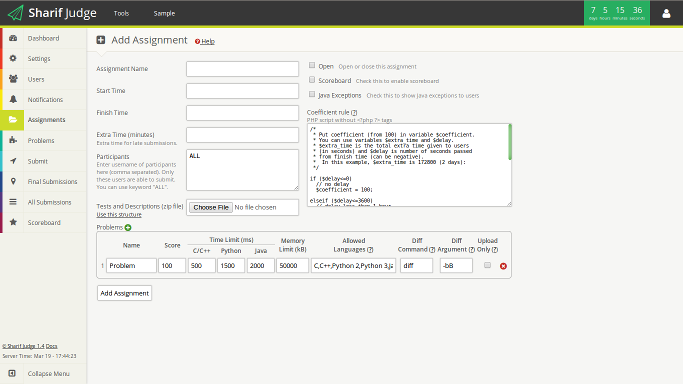
\includegraphics[width=1.0\textwidth]{add_assignment}  
	\caption[Tampilan Halaman \textit{Assignments}]{Tampilan Halaman \textit{Assignments}} 
	\label{fig:addass} 
\end{figure} 

Berikut beberapa pengaturan yang terdapat pada halaman \textit{Add Assignments}:
\begin{itemize}
	\item \textit{Assignment Name} \\
	\textit{Assignment} akan ditampilkan dengan nama ini dalam daftar \textit{assignment}.
	
	\item \textit{Start Time} \\
	\textit{Users} tidak dapat mengumpulkan \textit{assignment} sebelum \textit{"Start Time"}. Gunakan format ini untuk \textit{start time}: \textit{MM/DD/YYYY HH:MM:SS}. Contoh: \textit{08/31/2013 12:00:00}
	
	\item \textit{Finish Time, Extra Time}\\
	\textit{Users} tidak dapat mengumpulkan \textit{assignment} setelah \textit{Finish Time + Extra Time}. \textit{Assignment} yang telat akan dikalikan dengan koefisien tertentu. Pengguna harus menulis \textit{script} PHP untuk menghitung koefisien pada bidang \textit{"Coefficient Rule"}. Gunakan format berikut untuk \textit{finish time}: \textit{MM/DD/YYYY HH:MM:SS}. Contoh: \textit{08/31/2013 23:59:59}. Waktu ekstra harus dalam menit. Pengguna dapat menggunakan \textit{*}. Contoh \textit{120} (2 jam) atau \textit{48*60} (2 hari).
	
	\item \textit{Participants} \\
	Masukan \textit{username} dari partisipan disini. Gunakan tanda koma untuk memisah \textit{username} antar peserta. Hanya \textit{users} ini yang dapat mengumpulkan \textit{assignment}. Pengguna dapat menggunakan kata kunci \textit{ALL} untuk mengijinkan semua \textit{users} agar dapat mengumpulkan \textit{assignment}. Contoh: \textit{admin, instructor1 , instructor2 ,student1  ,   student2,student3 , student4}.
	
	\item \textit{Open} \\
	Pengguna dapat membuka atau menutup \textit{assignment} menggunakan pilihan ini. Jika pengguna menutup \textit{assignment}, \textit{non-student users} masih dapat mengumpulkan \textit{assignment}.
	
	\item Scoreboard \\
	Pengguna dapat mengaktifkan atau mematikan papan nilai dengan menggunakan pilihan ini.
	
	\item \textit{Java Exceptions}\\
	Pengguna dapat mengaktifkan dan mematikan \textit{java exceptions} yang ditunjukan kepada \textit{students}. Perubahan pada pilihan ini tidak berdampak pada kode yang sebelumnya sudah dinilai. Nama \textit{exception} akan muncul jika \textit{tester/java\_exceptions\_list} berisikan nama tersebut. Jika pengguna mengaktifkan fitur ini, kode di bawah ini akan ditampilkan kepada \textit{students} saat \textit{exception} dilemparkan: \newpage
	\begin{lstlisting}[basicstyle=\ttfamily, frame=single,
columns=fullflexible, keepspaces=true, breaklines=true]
Test 1
ACCEPT
Test 2
Runtime Error (java.lang.ArrayIndexOutOfBoundsException)
Test 3
Runtime Error (java.lang.ArrayIndexOutOfBoundsException)
Test 4
ACCEPT
Test 5
ACCEPT
Test 6
ACCEPT
Test 7
ACCEPT
Test 8
Runtime Error (java.lang.ArrayIndexOutOfBoundsException)
Test 9
Runtime Error (java.lang.StackOverflowError)
Test 10
Runtime Error (java.lang.ArrayIndexOutOfBoundsException)
\end{lstlisting}
	
	\item \textit{\textit{Coefficient Rule}} \\
	Pengguna dapat menulis \textit{script} PHP pada bagian ini. Pengguna harus memasukan koefisien (dari 100) pada variabel \textit{\$coefficient}. Pengguna dapat menggunakan variabel \textit{\$extra\_time} dan \textit{\$delay}. \textit{\$extra\_time} merupakan total waktu ekstra yang diberikan kepada \textit{users} dalam satuan detik dan \textit{\$delay} merupakan jumlah detik berlalu dari waktu selesai (bisa negatif). \textit{Script} PHP pada bagian ini tidak mengandung \textit{tags <?php , <? , ?>}. Berikut contoh \textit{\$extra\_time} 172800 (2 hari):
	\begin{lstlisting}[basicstyle=\ttfamily, frame=single,
columns=fullflexible, keepspaces=true, breaklines=true]
if ($delay<=0)
// no delay
$coefficient = 100;

elseif ($delay<=3600)
// delay less than 1 hour
$coefficient = ceil(100-((30*$delay)/3600));

elseif ($delay<=86400)
// delay more than 1 hour and less than 1 day
$coefficient = 70;

elseif (($delay-86400)<=3600)
// delay less than 1 hour in second day
$coefficient = ceil(70-((20*($delay-86400))/3600));

elseif (($delay-86400)<=86400)
// delay more than 1 hour in second day
$coefficient = 50;

elseif ($delay > $extra_time)
// too late
$coefficient = 0;
\end{lstlisting}
	
	\item \textit{Time Limit} \\
	Pengguna dapat mengatur batas waktu untuk menjalankan kode dalam satuan milisekon. \textit{Python} dan \textit{Java} biasanya lebih lambat dari \textit{C/C++}.	Oleh karena itu \textit{Python} dan \textit{Java} membutuhkan waktu yang lebih.
	
	\item \textit{Memory Limit} \\
	Pengguna dapat mengatur batas memori dalam satuan \textit{kilobyte}, namun penggunaan \textit{Memory Limit} tidak terlalu akurat.
	
	\item \textit{Allowed Languages} \\
	Pengguna dapat mengatur bahasa untuk setiap \textit{problem} (dipisahkan menggunakan koma). Bahasa yang tersedia seperti \textit{C, C++, Java, Python 2, Python 3, zip, PDF}. Pengguna dapat menggunakan \textit{zip} atau \textit{PDF} jika mengaktifkan pilihan \textit{Upload Only}. Contoh: \textit{C, C++ , zip} atau \textit{Python 2,Python 3} atau \textit{Java ,C}.
	
	\item \textit{Diff Command} \\
	\textit{Command} ini digunakan untuk membandingkan keluaran dengan keluaran yang benar. Secara \textit{default Sharif Judge} menggunakan \textit{diff}, namun pengguna dapat mengubah \textit{command} pada bagian ini.
	
	\item \textit{Diff Arguments} \\
	Pengguna dapat mengatur argumen dari \textit{Diff Command} disini. Untuk melihat daftar lengkap \textit{diff} argumen, pengguna dapat melihat \textit{man diff}. \textit{Sharif Judge} menambahkan dua pilihan baru yaitu \textit{ignore} dan \textit{identical}. \textit{Ignore} akan menghiraukan semua baris baru dan spasi. \textit{Identical} tidak akan menghiraukan apapun namun keluaran dari file yang dikumpulkan harus identik dengan keluaran \textit{test case} agar dapat diterima.
	
	\item \textit{Upload Only} \\
	Jika pengguna mengatur \textit{problem} sebagai \textit{Upload-Only}, maka \textit{Sharif Judge} tidak akan menilai \textit{assignment} pada \textit{problem} tersebut. Pengguna dapat menggunakan \textit{zip} dan \textit{PDF} pada \textit{allowed languages} jika mengaktifkan pilihan ini.
\end{itemize}

\subsubsection{Contoh \textit{Assignment}}

Berikut contoh \textit{assignment} untuk mencoba \textit{Sharif Judge}. Menambah \textit{assignment} dengan mengklik \textit{Add} di halaman \textit{Assignment}. \textit{Assignment} dibagi menjadi 3 \textit{problem}:
\begin{enumerate}
	\item \textit{Problem} 1 (Penjumlahan) \\
	Program pengguna akan menerima masukan bilangan \textit{integer} n, kemudian menerima masukan lagi sebanyak n buah bilangan \textit{integer} dan menampilkan hasil penjumlahan dari n nomor tersebut. Untuk lebih jelas, perhatikan tabel~\ref{tab:tablesum}.
	
	\begin{table}[H] %atau h saja untuk "kira kira di sini"
		\centering 
		\caption{\textit{Problem} 1 (Penjumlahan)}
		\label{tab:tablesum}
		\begin{tabular}{|c|c|}
			\hline
			Sample Input & Sample Output\\
			
			\hline
			\multicolumn{1}{|l|}{5} & \multirow{2}{*}{145}\\
			\multicolumn{1}{|l|}{54 78 0 4 9} & \\
			
			\hline
			
		\end{tabular} 
	\end{table}
	
	\item \textit{Problem} 2 (\textit{Max}) \\
	Program pengguna akan menerima masukan bilangan \textit{integer} n, kemudian menerima masukan lagi sebanyak n buah bilangan \textit{integer} dan menampilkan hasil penjumlahan dari dua nilai tertinggi. Untuk lebih jelas, perhatikan tabel~\ref{tab:tablemax}.
	
	\begin{table}[H] %atau h saja untuk "kira kira di sini"
		\centering 
		\caption{\textit{Problem} 2 (\textit{Max})}
		\label{tab:tablemax}
		\begin{tabular}{|c|c|}
			\hline
			Sample Input & Sample Output\\
			
			\hline
			\multicolumn{1}{|l|}{7} & \multirow{2}{*}{356}\\
			\multicolumn{1}{|l|}{162 173 159 164 181 158 175} & \\
			
			\hline
			
		\end{tabular} 
	\end{table}
	
	\item \textit{Problem} 2 (\textit{Upload!}) \\
	Pengguna diharuskan mengunggah sebuah \textit{file} \textit{C} atau \textit{zip}. \textit{Problem} ini menggunakan pilihan \textit{"Upload Only} sehingga tidak akan dinilai oleh \textit{Sharif Judge}.
\end{enumerate}

Pengguna dapat menemukan \textit{file zip} pada \textit{folder Assignments}. Perhatikan susunan pohon dari tugas ini:
\begin{lstlisting}[basicstyle=\ttfamily, frame=single,
columns=fullflexible, keepspaces=true, breaklines=true]
.
|-- p1
|   |-- in
|   |   |-- input1.txt
|   |   |-- input2.txt
|   |   |-- input3.txt
|   |   |-- input4.txt
|   |   |-- input5.txt
|   |   |-- input6.txt
|   |   |-- input7.txt
|   |   |-- input8.txt
|   |   |-- input9.txt
|   |   --- input10.txt
|   |-- out
|   |   --- output1.txt
|   |-- tester.cpp
|   --- desc.md
|-- p2
|   |-- in
|   |   |-- input1.txt
|   |   |-- input2.txt
|   |   |-- input3.txt
|   |   |-- input4.txt
|   |   |-- input5.txt
|   |   |-- input6.txt
|   |   |-- input7.txt
|   |   |-- input8.txt
|   |   |-- input9.txt
|   |   --- input10.txt
|   |-- out
|   |   |-- output1.txt
|   |   |-- output2.txt
|   |   |-- output3.txt
|   |   |-- output4.txt
|   |   |-- output5.txt
|   |   |-- output6.txt
|   |   |-- output7.txt
|   |   |-- output8.txt
|   |   |-- output9.txt
|   |   --- output10.txt
|   |-- desc.md
|   --- Problem2.pdf
|-- p3
|   --- desc.md
--- SampleAssignment.pdf
\end{lstlisting}
\textit{Problem} 1 menggunakan metode \textit{"Tester"} untuk mengecek keluaran, sehingga memiliki \textit{file tester.cpp (Tester Script)}. \textit{Problem} 2 menggunakan metode \textit{Output Comparison} untuk mengecek keluaran, sehingga memiliki dua \textit{folder} (\textit{in} dan \textit{out}) yang berisikan \textit{test case}. \textit{Problem} 3 merupakan \textit{problem} yang menggunakan pilihan \textit{Upload-Only}.

\subsubsection{Contoh Solusi}
\textit{Problem} diatas dapat diselesaikan menggunakan contoh solusi berikut ini:
\begin{itemize}
	\item Solusi \textit{Problem} 1 \\ 
	Menggunakan bahasa \textit{C}
	\begin{lstlisting}[basicstyle=\ttfamily, frame=single,
columns=fullflexible, keepspaces=true, breaklines=true]
#include<stdio.h>
int main(){
	int n;
	scanf("%d",&n);
	int i;
	int sum =0 ;
	int k;
	for(i=0 ; i<n ; i++){
		scanf("%d",&k);
		sum+=k;
	}
	printf("%d\n",sum);
		return 0;
}
\end{lstlisting} 
	
	
	Menggunakan bahasa \textit{C++}
	\begin{lstlisting}[basicstyle=\ttfamily, frame=single,
columns=fullflexible, keepspaces=true, breaklines=true]
#include <iostream>
using namespace std;
int main(){
	int n, sum=0;
	cin >> n;
	for (int i=0 ; i<n ; i++){
		int a;
		cin >> a;
		sum += a;
	}
	cout << sum << endl;
	return 0;
}
\end{lstlisting} 
	
	Menggunakan bahasa \textit{Java}
	\begin{lstlisting}[basicstyle=\ttfamily, frame=single,
columns=fullflexible, keepspaces=true, breaklines=true]
import java.util.Scanner;
class sum
{
	public static void main(String[] args)
	{ 
		Scanner sc = new Scanner(System.in);
		int n = sc.nextInt();
		int sum =0;
		for (int i=0 ; i<n ; i++)
		{
			int a = sc.nextInt();
			sum += a;
		}
		System.out.println(sum); 
	}
}
\end{lstlisting}
	
	\item Solusi \textit{Problem} 2 \\ 
	Menggunakan bahasa \textit{C}
	\begin{lstlisting}[basicstyle=\ttfamily, frame=single,
columns=fullflexible, keepspaces=true, breaklines=true]
#include<stdio.h>
int main(){
	int n , m1=0, m2=0;
	scanf("%d",&n);
	for(;n--;){
		int k;
		scanf("%d",&k);
		if(k>=m1){
			m2=m1;
			m1=k;
		}
		else if(k>m2)
			m2=k;
	}
	printf("%d",m1+m2);
	return 0;
}
\end{lstlisting}
	 
	
	Menggunakan bahasa \textit{C++}
	\begin{lstlisting}[basicstyle=\ttfamily, frame=single,
columns=fullflexible, keepspaces=true, breaklines=true]
#include<iostream>
using namespace std;
int main(){
	int n , m1=0, m2=0;
	cin >> n;
	for(;n--;){
		int k;
		cin >> k;
		if(k>=m1){
			m2=m1;
			m1=k;
		}
		else if(k>m2)
			m2=k;
		}
	cout << (m1+m2) << endl ;
	return 0;
}
\end{lstlisting}
\end{itemize}

\subsection{Struktur Pengujian}

Pengguna harus menyediakan sebuah \textit{file zip} yang berisikan \textit{test cases} ketika menambahkan \textit{assignment}. \textit{File zip} ini dapat berisikan folder-folder untuk setiap \textit{problem}. Pengguna harus memberikan nama pada folder sesuai aturan seperti \textit{p1, p2, p3, dst}. \textit{Assignment} yang menggunakan pilihan \textit{Upload-Only} tidak membutuhkan \textit{folder}~\cite{mjnaderi:14:sharifjudgedoc}.

\subsubsection{Metode Pengecekan}
\textit{Sharif Judge} memiliki dua metode pengecekan untuk setiap \textit{problem} yaitu metode \textit{"Input/Output" Comparison} dan metode \textit{Tester}.
\begin{itemize}
	\item \textit{Metode Input/Output Comparison} \\
	Dengan metode ini, pengguna harus memasukan beberapa \textit{file input dan output} pada \textit{folder} \textit{problem}. \textit{Sharif Judge} akan memasukan nilai dari \textit{file input} ke kode \textit{users} dan membandingkan hasil keluaran dari kode \textit{users} dengan \textit{file output}. \textit{Input files} harus berada dalam folder \textit{"in"} dengan nama \textit{input1.text, input2.txt, dst}.\textit{Output files} harus berada dalam folder \textit{"out"} dengan nama \textit{output1.txt, output2.txt, dst}.
	
	\item \textit{Metode Tester} \\
	Dengan metode ini, pengguna harus menyediakan beberapa \textit{file input} dan sebuah \textit{file C++ (tester.cpp)} dan beberapa \textit{file output}. \textit{Sharif Judge} akan memasukan nilai dari \textit{file input} ke kode \textit{users} dan mengambil keluaran dari kode \textit{users}. \textit{tester.cpp} akan mengambil nilai dari \textit{file input, file output, }dan keluaran \textit{users}. Jika keluaran dari kode \textit{users} benar akan mengembalikan nilai 0, sebaliknya jika salah akan mengeluarkan nilai 1. Berikut contoh kode untuk menulis \textit{tester.cpp}:
	\begin{lstlisting}[basicstyle=\ttfamily, frame=single,
columns=fullflexible, keepspaces=true, breaklines=true]
/*
* tester.cpp
*/

#include <iostream>
#include <fstream>
#include <string>
using namespace std;
int main(int argc, char const *argv[])
{
	
	ifstream test_in(argv[1]);  /* Stream ini membaca 
	isi file input */
	ifstream test_out(argv[2]); /* Stream ini membaca 
	isi file output */
	ifstream user_out(argv[3]); /* Stream ini membaca 
	isi keluaran users */
	
	/* Kode Pengguna */
	/* Jika keluaran kode user benar, mengembalikan nilai 0, 
	sebaliknya mengembalikan 1 */
	
	...

}
\end{lstlisting}
\end{itemize}

\subsubsection{Contoh \textit{File}}

Pengguna dapat menemukan contoh \textit{file} penguji pada \textit{folder Assignments}. Perhatikan susunan pohon dari \textit{file} tersebut:
\begin{lstlisting}[basicstyle=\ttfamily, frame=single,
columns=fullflexible, keepspaces=true, breaklines=true]
.
|-- p1
|   |-- in
|   |   |-- input1.txt
|   |   |-- input2.txt
|   |   |-- input3.txt
|   |   |-- input4.txt
|   |   |-- input5.txt
|   |   |-- input6.txt
|   |   |-- input7.txt
|   |   |-- input8.txt
|   |   |-- input9.txt
|   |   --- input10.txt
|   |-- out
|   |   --- output1.txt
|   --- tester.cpp
--- p2
	|-- in
	|   |-- input1.txt
	|   |-- input2.txt
	|   |-- input3.txt
	|   |-- input4.txt
	|   |-- input5.txt
	|   |-- input6.txt
	|   |-- input7.txt
	|   |-- input8.txt
	|   |-- input9.txt
	|   --- input10.txt
	--- out
	|-- output1.txt
	|-- output2.txt
	|-- output3.txt
	|-- output4.txt
	|-- output5.txt
	|-- output6.txt
	|-- output7.txt
	|-- output8.txt
	|-- output9.txt
	--- output10.txt
\end{lstlisting}

\textit{Problem} 1 menggunakan metode \textit{"Tester"} untuk mengecek hasil keluaran, sehingga memiliki \textit{file tester.cpp}. Berikut isi dari \textit{file tester.cpp} untuk \textit{problem} 1:
\begin{lstlisting}[basicstyle=\ttfamily, frame=single,
columns=fullflexible, keepspaces=true, breaklines=true]
/*
* tester.cpp
*/

#include <iostream>
#include <fstream>
#include <string>
using namespace std;
int main(int argc, char const *argv[])
{
	
	ifstream test_in(argv[1]);  /* Stream ini membaca 
	isi file input */
	ifstream test_out(argv[2]); /* Stream ini membaca 
	isi file output */
	ifstream user_out(argv[3]); /* Stream ini membaca 
	isi keluaran users */
	
	/* Kode Pengguna */
	/* Jika keluaran kode user benar, mengembalikan nilai 0, 
	sebaliknya mengembalikan 1 */
	/* e.g.: Permasalahan: membaca n nomor dan keluarkan 
	hasil penjumlahannya: */
	
	int sum, user_output;
	user_out >> user_output;
	
	if ( test_out.good() ) // if test's output file exists
	{
		test_out >> sum;
	}
	else
	{
		int n, a;
		sum=0;
		test_in >> n;
		for (int i=0 ; i<n ; i++){
			test_in >> a;
			sum += a;
		}
	}
	
	if (sum == user_output)
		return 0;
	else
		return 1;

}
\end{lstlisting}


\textit{Problem} 2 menggunakan metode \textit{"Input/Output Comparison"} untuk mengecek hasil keluaran, sehingga memiliki dua folder \textit{in} dan \textit{out} yang berisikan \textit{test cases}. \textit{Problem} 3 menggunakan pilihan \textit{Upload-Only}, sehingga tidak memiliki folder apapun.

\subsection{Deteksi Kecurangan}
\textit{Sharif Judge} menggunakan \textit{Moss} untuk mendeteksi kode yang mirip. \textit{Moss (Measure Of Software Similarity)} merupakan sistem otomatis untuk menentukan kemiripan program. Pada saat ini, aplikasi utama \textit{Moss} telah digunakan untuk mendeteksi plagiarisme pada kelas \textit{programming}. Pengguna dapat mengirimkan kode final (yang dipilih oleh \textit{students} sebagai \textit{Final Submission}) ke \textit{server Moss} dengan satu klik~\cite{mjnaderi:14:sharifjudgedoc}.\\

Sebelum menggunakan \textit{Moss} ada beberapa hal yang harus diperhatikan yaitu:
\begin{itemize}
	\item Pengguna harus mendapatkan \textit{Moss user id} dan mengaturnya di \textit{Sharif Judge}. Untuk mendapatkan \textit{Moss user id}, pengguna harus terlebih dahulu daftar pada halaman \path{http://theory.stanford.edu/~aiken/moss/}. Pengguna akan mendapatkan sebuah \textit{email} yang berisikan \textit{script perl}. \textit{Moss user id} berada pada \textit{script} tersebut. \\
	Berikut potongan \textit{perl script} yang berisikan \textit{user id}:

\begin{lstlisting}[basicstyle=\ttfamily, frame=single,
columns=fullflexible, keepspaces=true, breaklines=true]
...

$server = 'moss.stanford.edu';
$port = '7690';
$noreq = "Request not sent.";
$usage = "usage: moss [-x] [-l language] [-d] 
		  [-b basefile1] ... [-b basefilen] [-m #] 
		  [-c \"string\"] file1 file2 file3 ...";

#
# The userid is used to authenticate your queries to the server; 
  don't change it!
#
$userid=YOUR_MOSS_USER_ID;

#
# Process the command line options.  This is done in a non-standard
# way to allow multiple -b's.
#
$opt_l = "c";   # default language is c
$opt_m = 10;
$opt_d = 0;

...
}

\end{lstlisting}

\item Dapatkan \textit{user id} tersebut lalukan gunakan pada \textit{Sharif Judge} untuk mendetksi kecurangan. Pengguna dapat menyimpan \textit{user id} di \textit{Sharif Judge} pada halaman \textit{Moss}. \textit{Sharif Judge} akan menggunakan \textit{user id} tersebut di \textit{Moss perl script}.

\item \textit{Server} pengguna harus menginstal \textit{perl} untuk menggunakan \textit{Moss}.

\item Pengguna dianjurkan untuk mendetek kode yang mirip setelah waktu \textit{assignment} berakhir, karena para peserta masih dapat mengubah \textit{Final Submissions} masing-masing sebelum waktu habis. Dengan cara tersebut \textit{Sharif Judge} dapat mengirimkan \textit{Final submissions} para peserta ke \textit{server Moss}.
\end{itemize}
